\chapter{Partie algorithmique : analyse du problème}

\section{Différentes compétences}
Au cours de ce projet, nous avons acquis une série de compétences essentielles en programmation et en gestion de projet. Ces compétences incluent non seulement la création et la gestion de documents, l'utilisation des outils de développement, mais également la gestion collaborative du code et la mise en place de bonnes pratiques de développement.

Chaque membre de l’équipe a appris à utiliser les commandes de base de Git, telles que \texttt{git add}, \texttt{git commit}, \texttt{git push} et \texttt{git pull}, ce qui a permis de maintenir un répertoire centralisé et d’éviter les conflits de code. Cela nous a également permis de travailler en parallèle sur des parties distinctes du code, tout en maintenant une communication constante sur l’avancement des tâches et les problèmes rencontrés. 

\textbf{Développement du code en C :} Le développement en langage C a été au cœur de notre projet. Nous avons créé et structuré différents fichiers sources \texttt{.c} et \texttt{.h}, en respectant des principes de modularité et de réutilisation de code. Chaque fonction implémentée a été testée pour répondre aux contraintes liées à la résolution du labyrinthe. Nous avons fait le choix d'utiliser de nombreux types : les listes, les listes chaînées, les ensembles et les piles afin de faciliter ensuite l'implémentation des fonctions essentielles à la résolution du labyrinthe. 

\textbf{Tests et correction :} Pour nous assurer de la fiabilité de notre code, nous avons mis en place une série de tests unitaires. Ces tests ont permis de valider le bon fonctionnement des différentes fonctions développées, ainsi que de détecter et corriger d'éventuels bugs. 

\textbf{Respect des conventions de codage et collaboration :} Un autre aspect essentiel de notre travail en équipe a été le respect des conventions de codage, notamment en termes d’espace de nommage et de lisibilité du code.

\section{Types abstraits de données}
Afin de résoudre le problème du plus court chemin, il nous a semblé judicieux de créer des types nous permettant de manipuler un labyrinthe le plus simplement possible. Après de nombreuses discussions, le groupe a choisi de représenter les types suivants :\\

Les TAD Pile, Liste, Ensemble sont les mêmes que ceux explicités en cours. On considère, sans plus de démonstration, les types fondamentaux suivants:

\begin{itemize}
    \item \textbf{Direction} = \{H, B, G, D\}
    \item \textbf{Ordre} = \{AV, TD, TG\}
\end{itemize}
\vspace{5mm}
Dans la suite, 2 TAD vont être explicités (le TAD Labyrinthe et le TAD CaseEtDirection), détaillant les opérations possibles sur ces types.

\subsection{Labyrinthe}

\begin{tad}
	\tadNom{Labyrinthe}
	\tadDependances{\naturelNonNul, Direction, Ensemble}
    
	\begin{tadOperations}{}
        \tadOperationAvecPreconditions{labyrinthe}{\tadTroisParams{\naturelNonNul}{\naturelNonNul}\\{\naturelNonNul}}{\tadUnParam{\Labyrinthe}}
        \tadOperationAvecPreconditions{casserMur}{\tadTroisParams{\Labyrinthe}{\naturelNonNul}\\{\naturelNonNul}}{\tadUnParam{\Labyrinthe}}
        \tadOperation{largeur}{\tadUnParam{\Labyrinthe}}{\tadUnParam{\naturelNonNul}}
        \tadOperation{caseDEntree}{\tadUnParam{\Labyrinthe}}{\tadUnParam{\naturelNonNul}}
        \tadOperation{caseDeSortie}{\tadUnParam{\Labyrinthe}}{\tadUnParam{\naturelNonNul}}
        \tadOperation{directionsPossible}{\tadDeuxParams{\Labyrinthe}\\{\naturelNonNul}}{\tadUnParam{Ensemble<Direction>}}
        \tadOperationAvecPreconditions{caseDestination}{\tadTroisParams{\Labyrinthe}{\naturelNonNul}\\{Direction}}{\tadUnParam{\naturelNonNul}}
        \tadOperationAvecPreconditions{casesAdjacentes}{\tadDeuxParams{\Labyrinthe}\\{\naturelNonNul}}{\tadUnParam{Ensemble<\naturelNonNul>}}
        \tadOperationAvecPreconditions{casesAccessibles}{\tadDeuxParams{\Labyrinthe}\\{\naturelNonNul}}{\tadUnParam{Ensemble<\naturelNonNul>}}
        \tadOperationAvecPreconditions{casesNonAccessibles}{\tadDeuxParams{\Labyrinthe}\\{\naturelNonNul}}{\tadUnParam{Ensemble<\naturelNonNul>}}
        \tadOperation{directionEntreeEtSortie}{\tadUnParam{\Labyrinthe}}{\tadDeuxParams{Direction}\\{Direction}}
	\end{tadOperations}

	\begin{tadSemantiques}{}
        \tadSemantique{labyrinthe}{L'opération qui permet de créer un labyrinthe muré de taille \(n^2\).}
        \tadSemantique{casserMur}{L'opération qui permet de créer un accès d'une case à une autre.}
        \tadSemantique{largeur}{L'opération qui permet de renvoyer la largeur n d'un labyrinthe.}
        \tadSemantique{caseDEntree}{L'operation qui permet de renvoyer la case d'entrée du labyrinthe.}
        \tadSemantique{caseDeSortie}{L'opération qui permet de renvoyer la case de sortie du labyrinthe.}
        \tadSemantique{directionsPossible}{L'opération qui permet de renvoyer les directions
        possibles depuis une case.}
        \tadSemantique{caseDestination}{L'opération qui permet de renvoyer la case d'arrivée après l'emprunt de la direction depuis la case précédente.}
        \tadSemantique{casesAdjacentes}{L'opération qui permet de renvoyer les cases adjacentes à une case.}
        \tadSemantique{casesAccessibles}{L'opération qui permet de renvoyer les cases accessibles depuis une case.}
        \tadSemantique{casesNonAccessibles}{L'opération qui permet de renvoyer les cases non accessibles depuis une case.}
        \tadSemantique{directionEntreeEtSortie}{L'opération qui permet de renvoyer les directions des portes d'entrée et de sortie du labyrinthe.}
        \end{tadSemantiques}

	\begin{tadPreconditions}{}
        \tadPrecondition{labyrinthe}{entree \(\neq\) sortie,\\ \(entree \in [|1,n|] \cup [|n^2-n,n^2|] \cup \{k \in [|1,n|] \mid k \times n\} \cup \{k \in [|1,n|] \mid k \times n + 1\}\)\\
        \(sortie \in [|1,n|] \cup [|n^2-n,n^2|] \cup \{k \in [|1,n|] \mid k \times n\} \cup \{k \in [|1,n|] \mid k \times n + 1\}\)}
        \tadPrecondition{casserMur}{c1 \(\neq\) c2, \(c1 \leq largeur(l)^2\) et \(c2 \leq largeur(l)^2\)}
        \tadPrecondition{caseDestination}{\texttt{estPresent(directionsPossible(l,c),d)}}
        \tadPrecondition{casesAdjacentes}{\(c \leq largeur(l)^2\)}
        \tadPrecondition{casesAccessibles}{\(c \leq largeur(l)^2\)}
        \tadPrecondition{casesNonAccessibles}{\(c \leq largeur(l)^2\)}
	\end{tadPreconditions}
	
\end{tad}


 
\subsection{Case et direction}

\begin{tad}
	\tadNom{caseEtDirection}
	\tadDependances{\naturelNonNul, Direction}
    
	\begin{tadOperations}{}
        \tadOperation{creerCaseEtDirection}{\tadDeuxParams{\naturelNonNul}\\{Direction}}{\tadUnParam{caseEtDirection}}
        \tadOperationAvecPreconditions{fixerCase}{\tadDeuxParams{caseEtDirection}\\{\naturelNonNul}}{\tadUnParam{caseEtDirection}}
        \tadOperation{fixerDirection}{\tadDeuxParams{caseEtDirection}\\{Direction}}{\tadUnParam{caseEtDirection}}
        \tadOperation{obtenirCase}{\tadUnParam{caseEtDirection}}{\tadUnParam{\naturelNonNul}}
        \tadOperation{obtenirDirection}{\tadUnParam{caseEtDirection}}{\tadUnParam{Direction}}
	\end{tadOperations}
	
	\begin{tadSemantiques}{}
        \tadSemantique{creerCaseEtDirection}{L'opération qui permet de créer\\un objet de type caseEtDirection.}
        \tadSemantique{fixerCase}{L'opération qui permet d'attribuer une case à un objet de type caseEtDirection.}
        \tadSemantique{fixerDirection}{L'opération qui permet d'attribuer\\une direction à un objet de type caseEtDirection.}
        \tadSemantique{obtenirCase}{L'opération qui permet de renvoyer la case\\associée à un objet de type caseEtDirection.}
        \tadSemantique{obtenirDirection}{L'opération qui permet de renvoyer\\la direction associée à un objet de type caseEtDirection.}
        \end{tadSemantiques}

	\begin{tadPreconditions}{}
        \tadPrecondition{fixerCase}{\(c \leq largeur(l)^2\)}
	\end{tadPreconditions}

\end{tad}

 
 

\section{Analyses descendantes}
L'analyse descendante consiste à diviser un problème complexe en\\ sous-problèmes plus simples, et ainsi de suite, jusqu'à obtenir des éléments\\ suffisamment simples pour être résolus directement.
Pour ce projet, nous avons mis en place deux analyses descendantes, une pour la partie algorithmique du projet, l'autre pour la partie électronique. Celles-ci sont disponibles plus amplement en annexe.
\vspace{0.10cm}

\begin{figure}[htbp]
    \centering
    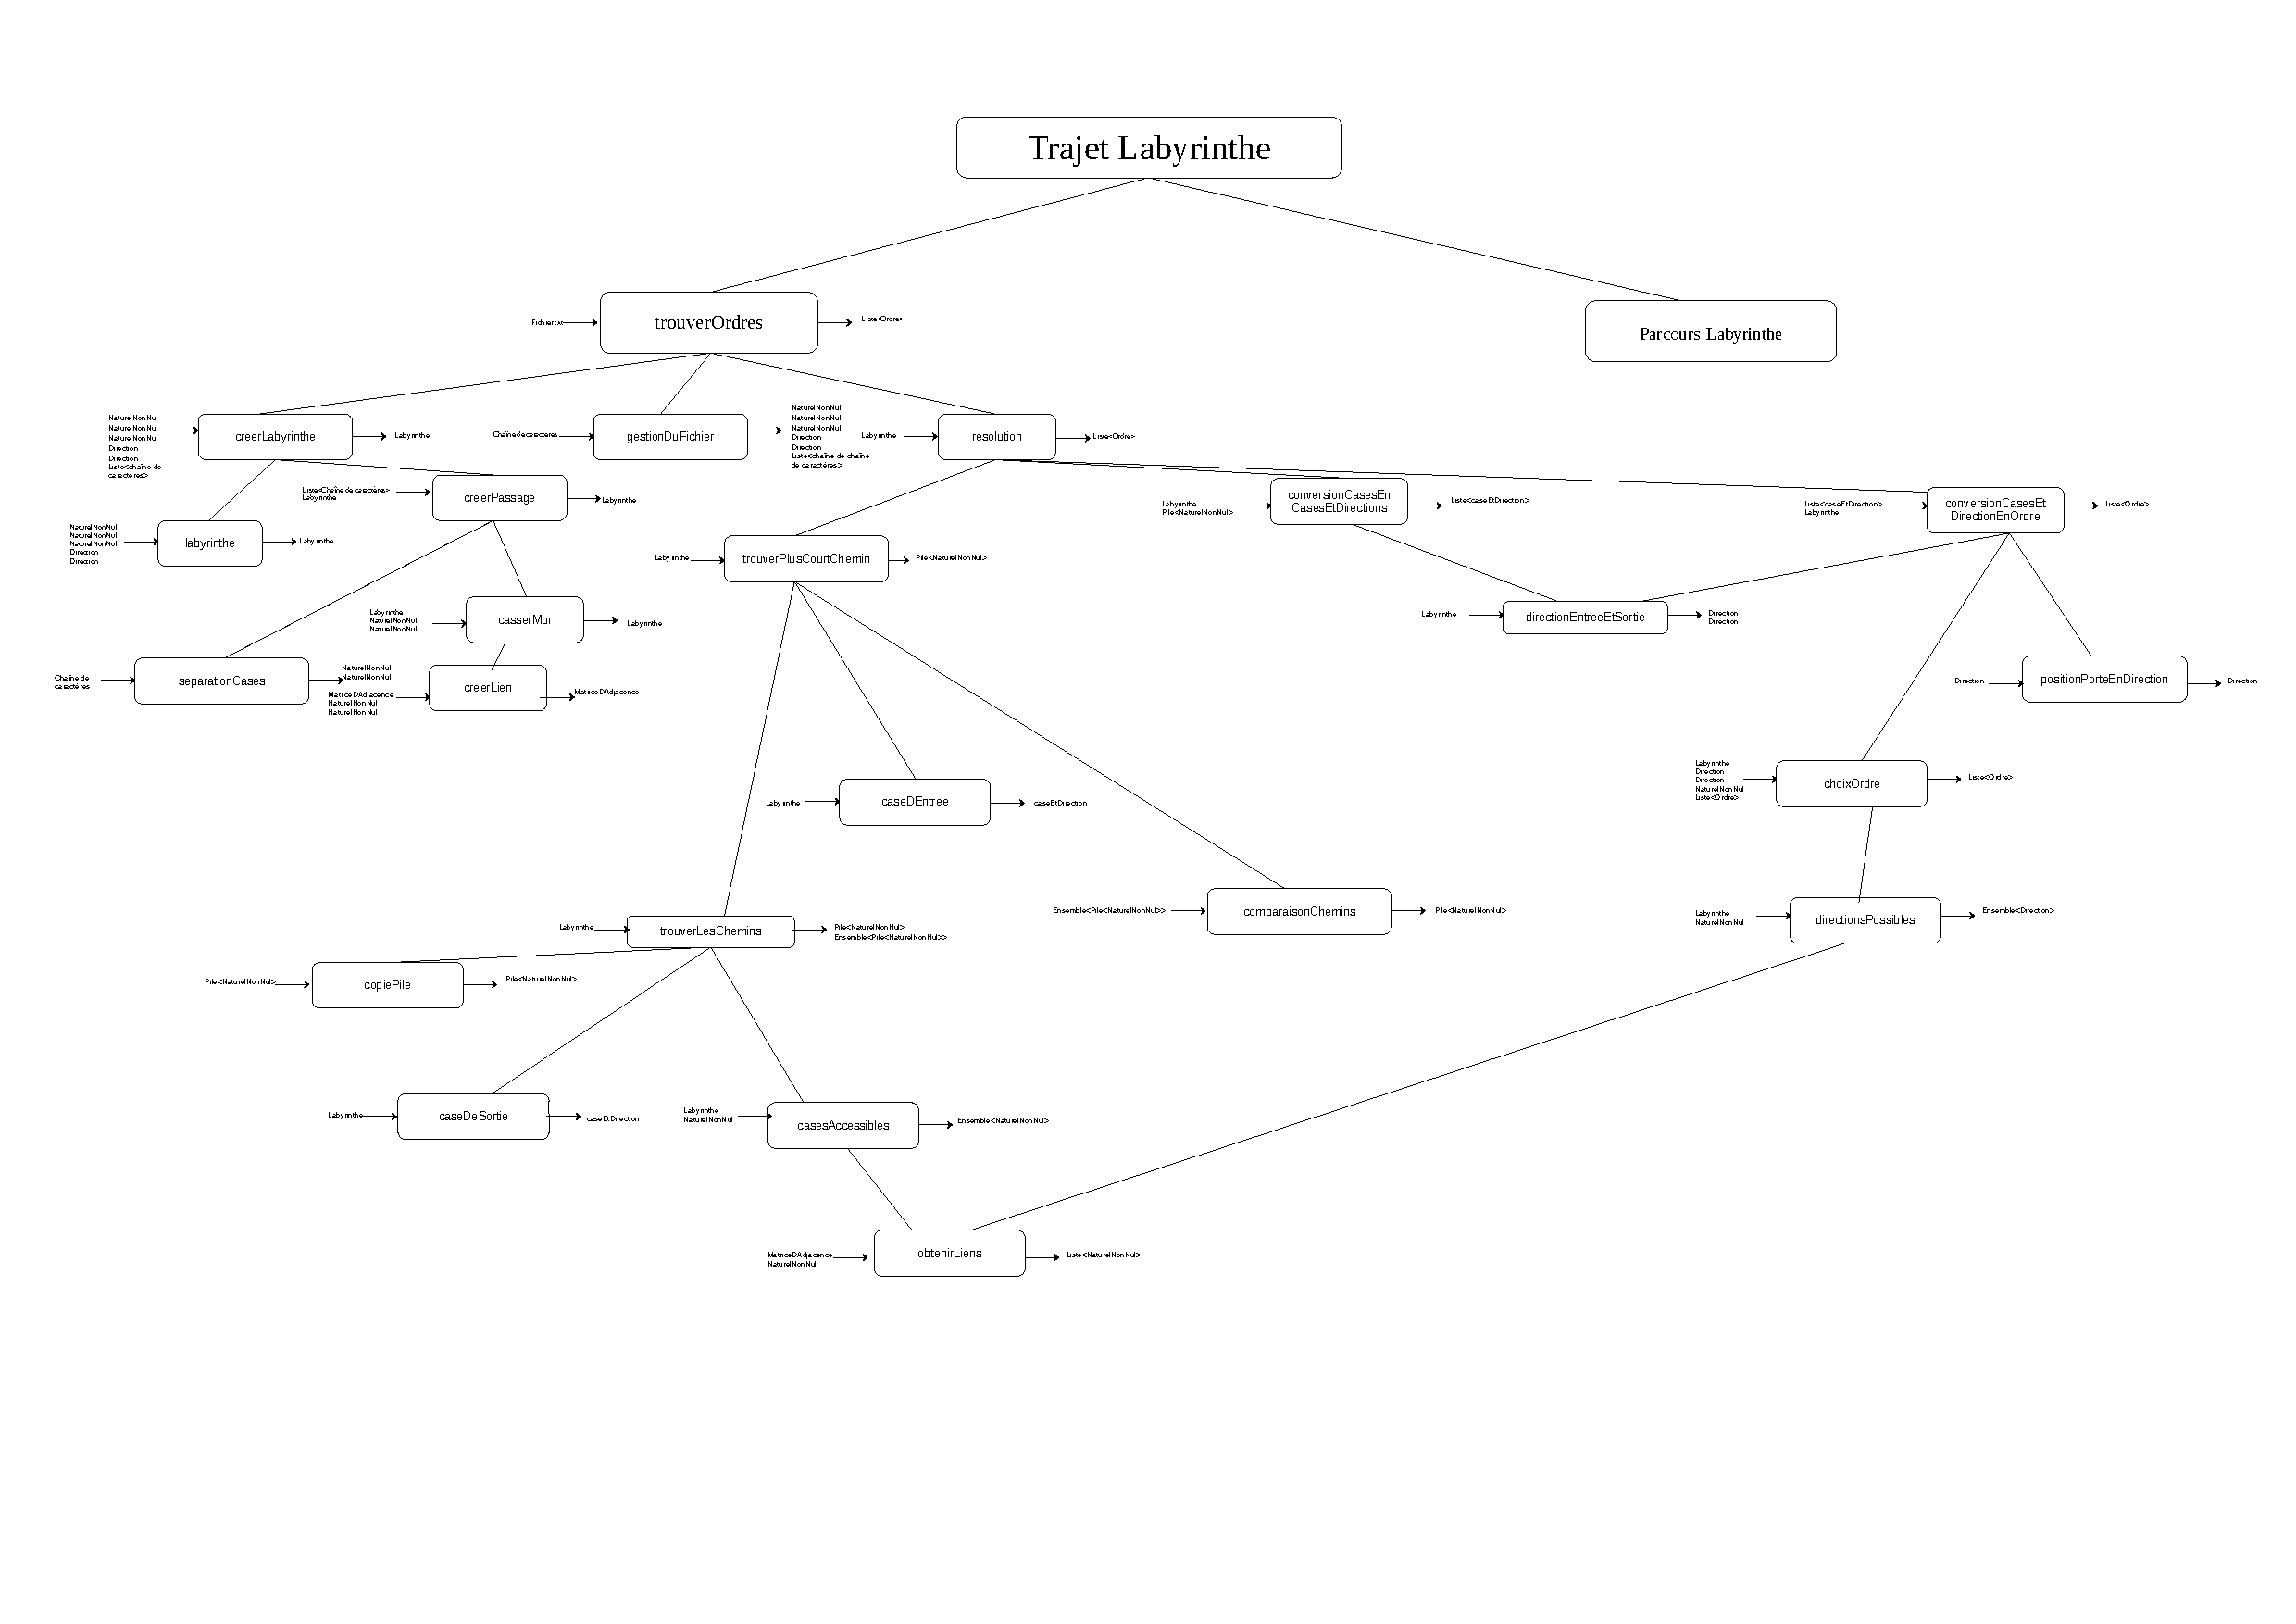
\includegraphics[width=1.2\textwidth]{algo/analyse/analyseDescendante_Algo.pdf} 
    \caption{Analyse descendante de la partie algorithmique}
    \label{fig:analyse}
\end{figure}


\begin{figure}[htbp]
    \centering
    \caption{Analyse descendante de la partie électronique} 
    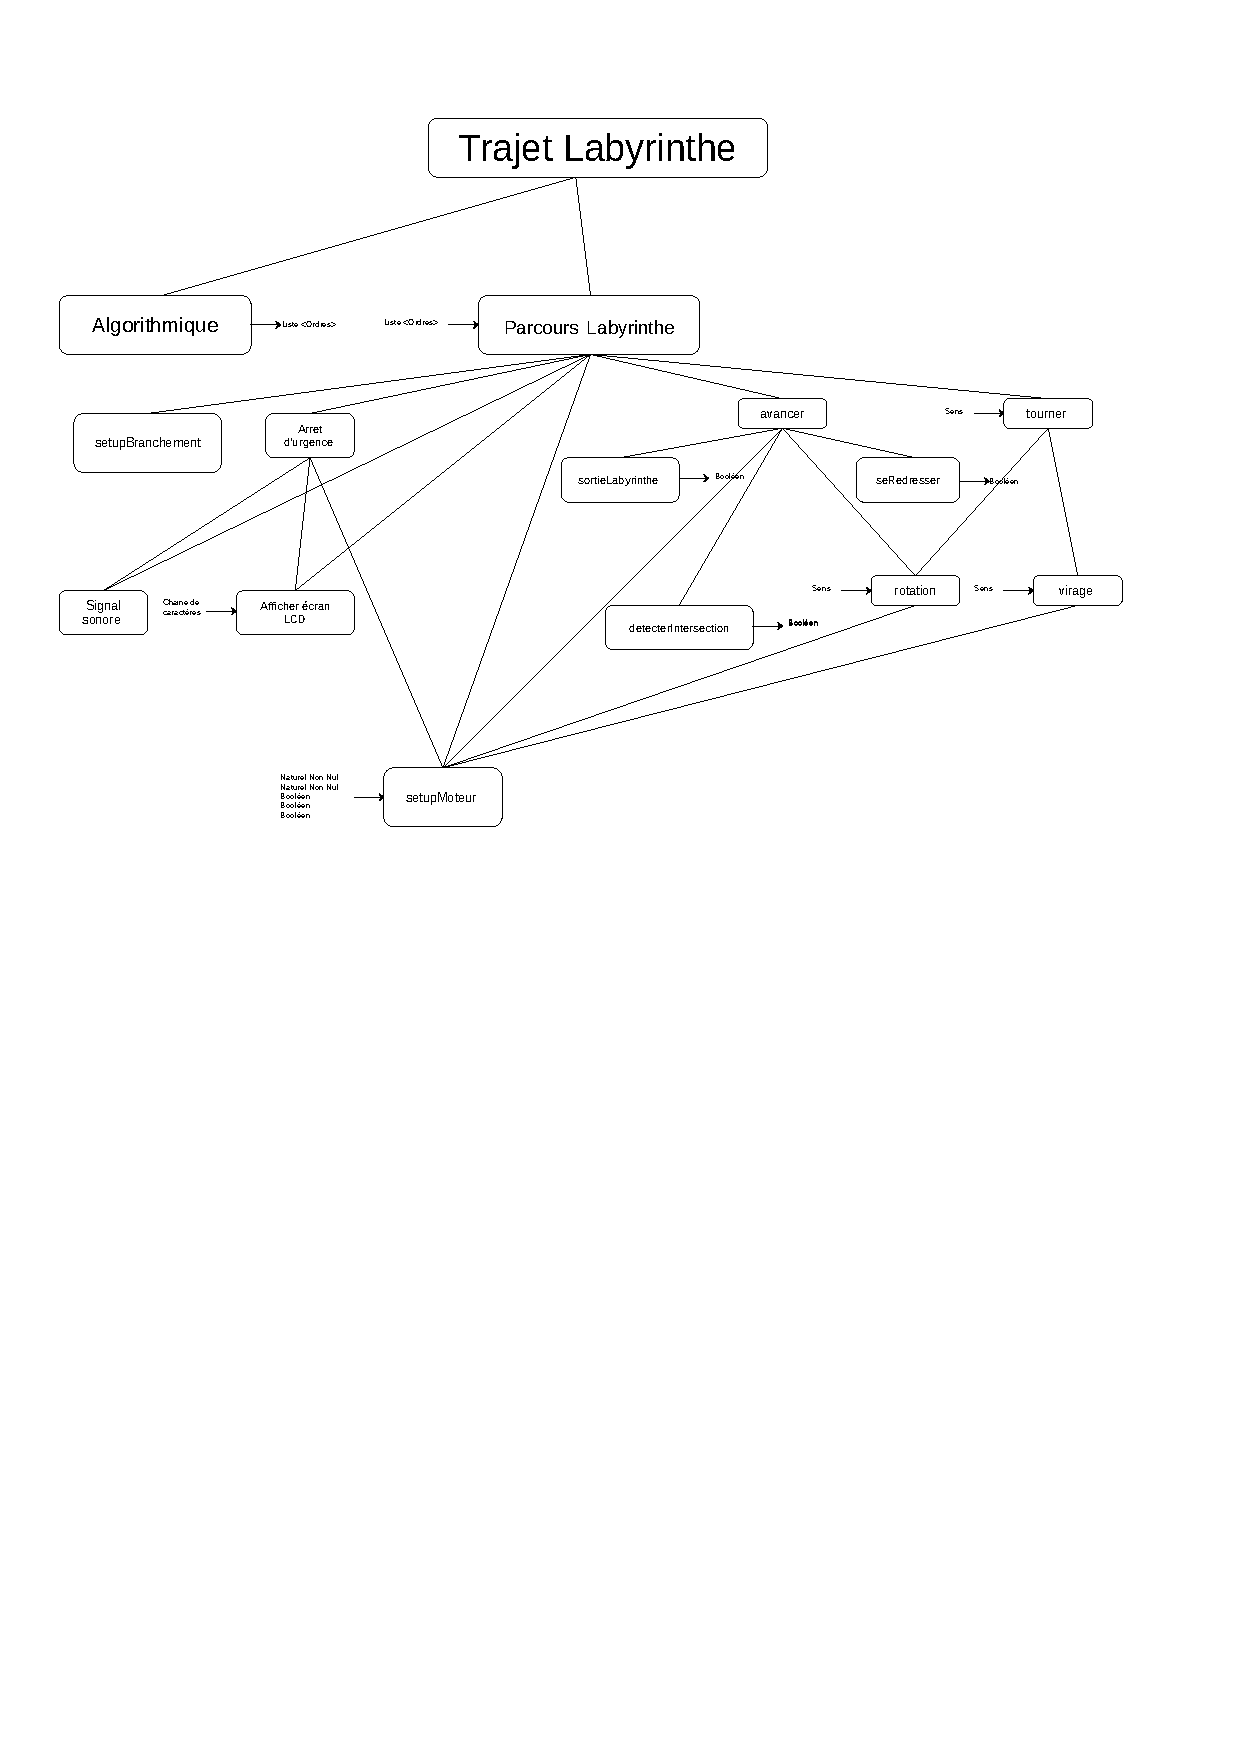
\includegraphics[width=1.2\textwidth]{elec/analyseDescendante_Elec.pdf}  
    \label{fig:analyse}
\end{figure}
